%%%%%%%%%%%%%%%%%%%%%%%%%%%%%% Preamble
\documentclass[11pt]{article}
\setlength{\parskip}{\baselineskip}%
\setlength{\parindent}{0pt}%
\usepackage{amsmath,amssymb,amsthm,physics,graphicx,titling,hyperref}
\usepackage[margin=0.4in]{geometry}
\newcommand{\subtitle}[1]{%
  \posttitle{%
    \par\end{center}
    \begin{center}\large#1\end{center}
    \vskip0.5em}%
}

\begin{document}

%%%%%%%%%%%%%%%%%%%%%%%%%%%%%% Heading
	\title{Ph21 Assignment 3 - Image Processing}
	\author{Yovan Badal}
	\date{05/20/2018}
	\maketitle
	
%%%%%%%%%%%%%%%%%%%%%%%%%%%%%% Body
\section{Procedure}
We implement the Canny edge detector using the PIL library to extract RGB arrays from images, and the scipy ndimage library for image processing. We sum over the RGB values of each pixel to obtain an array of brightness values, with which we convolve the first derivative of a Gaussian kernel by using ndimage's \textit{gaussian\_gradient\_magnitude}. This stencil is applied and $\sigma$ is varied to optimize for edge detection, where $\sigma$ is the width parameter of the distribution (how many neighboring pixels are used to compute the gradient at a given pixel).

\begin{figure}[!htbp]
\centering
  \begin{minipage}[b]{0.3\textwidth}
    
\includegraphics[width=\textwidth]{procrastination.png}
  \end{minipage}
   \begin{minipage}[b]{0.3\textwidth}
    
\includegraphics[width=\textwidth]{sigma4_procrastination.png}
  \end{minipage}
  
   \begin{minipage}[b]{0.3\textwidth}
    
\includegraphics[width=\textwidth]{sigma8_procrastination.png}
  \end{minipage}
   \begin{minipage}[b]{0.3\textwidth}
    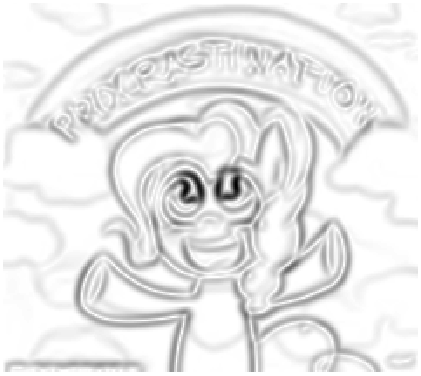
\includegraphics[width=\textwidth]{sigma20_procrastination.png}
  \end{minipage}
  \caption{Edge detection on sample image (top left) with from top right to bottom right, $\sigma=0.4, 0.8, 2.0$.}
\end{figure}

\section{Limitations}
\subsection{Pure RGB images}
We detect edges using the magnitude of the brightness gradient (red+green+blue values). Therefore, we expect our algorithm to be unable to detect edges composed only color transitions (for example, a transition between a pure red region (255, 0, 0) to a pure green region (0, 255, 0) with no change in brightness). However, in real world situations, edges correspond to a change in brightness. In fact, even seemingly pure RGB images are constructed with small changes in brightness to make them look more natural.

\begin{figure}[!htbp]
  \begin{minipage}[b]{0.5\textwidth}
    
\includegraphics[width=\textwidth]{flag.png}
    \caption{Mauritian flag}
  \end{minipage}
  \hfill
  \begin{minipage}[b]{0.5\textwidth}
    
\includegraphics[width=\textwidth]{sigma4_flag.png}
    \caption{Edge detection with $\sigma = 0.4$}
  \end{minipage}
\end{figure}

\subsection{Double detection}
We observe double-edges in our test image (Figure 1). To avoid these double detections, we could make use of edge-thinning algorithms relying on connectivity tests. One popular algorithm to do this is the 8-connectivity test, whereby all nearest-neighbors of an edge pixel are considered: for each direction from a pixel to a nearest neighbor, the pixel is removed if the pixel has no neighbor in that direction, is not the end of a line, and is isolated. The algorithm is iterated over several passes for each direction.

\subsection{CAPTCHAs}
Edge-detection alone cannot be used to beat CAPTCHA's, as most CAPTCHAs don't rely on using a background to fool OCR software (otherwise we could in fact use edge detection and pass the output to OCR). Some CAPTCHAs rely on warping letters, such that OCR is unable to recognize characters. This is very difficult to do without human interpretation or prohibitively resource-consuming machine-learning algorithms. Furthermore, modern CAPTCHAs rely directly on image recognition (e.g. identifying images containing a Stop sign), which is a much harder computer vision problem than edge detection.
\end{document}